% Seminar Thesis Template - Chair for High-Performance Computing
% Note: If you write your thesis in German, then change the babel package include
%       to "ngerman".
%
% TODOs:
% 1. Configure the seminar thesis options (title, author, ...) in "my_config.tex".
% 2. If the language of your thesis is not English: Change the option in the babel
%    package import to "ngerman". (see below)
% 3. (Optional) You might want to switch the BibLaTeX backend from "bibtex" to "biber".
%
\documentclass[10pt,          % font size
               a4paper,       % page layout
               twocolumn,     % two-column format
               DIV=14,        % page margins
               BCOR=8mm,      % binding correction for two-sided prints
               twoside        % for two-sided prints
              ]{scrartcl}

% TODO: Set language here
\usepackage[english]{babel}   % change to "ngerman" if you write your thesis in German

\usepackage{hpcseminar}
\usepackage[utf8]{inputenc}   % UTF-8 encoding (for umlauts etc.)
\usepackage[T1]{fontenc}      % correct hyphenation
\usepackage{csquotes}         % correct quotation marks
\usepackage{lmodern}          % Computer Modern fonts
\usepackage{microtype}        % better typesetting results (avoids underfull / overfull hboxes)
\usepackage{graphicx}         % adding graphics
\usepackage{units}            % typesetting units, e.g. \unit[10]{MB} and \unitfrac[100]{Mbit}{s}
\usepackage{booktabs}         % publication quality tables
%\usepackage{siunitx}         % alternative (more features) unit typesetting package


% BibLaTeX settings
\usepackage[backend=bibtex, style=numeric, maxcitenames=2, natbib=true]{biblatex}
\addbibresource{literature}

% Put your own includes in "my_includes.tex"
% Platz f\"{u}r eigene Erweiterungen und Definitionen

%\usepackage{XYZ}
%\newcommand{\hi}{Hallo}
\usepackage{subcaption}



\begin{document}

%% TODO: Configure details in my_config.tex
%% Ein paar wichtige Details konfigurieren
%%----------------------------------------
\title{Visualization of Data Movements and Accesses}
\author{Til Mohr}
\supervisor{Isa Thärigen, M.Sc.}
\semester{Summer Term 2023}
\keywords{data locality, data movement, data access, optimization, visualization}%TODO


% Generate title
\maketitle

% Abstract
% TODO: Write your abstract in "abstract.tex"
\begin{abstract}
\noindent The widening processor-memory performance gap and the increasing complexity of programs necessitate better data locality optimization methods for efficient computation. This paper presents a comprehensive overview of visualization techniques for data movements and accesses to aid in data locality optimization. It includes methods of data gathering like dynamic analysis, static analysis, and simulation, and discusses their usage in various visualization tools at different granularities. Three specific tools are detailed, providing unique perspectives on data movement visualization. The paper further outlines the standard performance optimization workflow and provides an outlook on future enhancements in data gathering, visualizations, and automated program optimization.

% Print out keywords
\noindent\keywordsline
\end{abstract}

% Chapters are included here
% TODO: Add your chapters in "my_chapters.tex"
% Sections / Chapters are included here
% Include your own sections / chapters if needed
\section{Introduction}\label{sec:introduction}
The pursuit of performance optimization in the field of high-performance computing (HPC) continues to push boundaries, with significant emphasis being placed on mitigating the impact of the increasing Processor-Memory Speed Gap and the rising computational memory requirements. These challenges are amplified by the escalating complexity of modern programs, making it increasingly difficult for experts to form a mental model of a program's data movement, let alone domain researchers. This complexity has led to a marked surge in the costs of data movement and the appearance of severe performance bottlenecks. While advancements in hardware can alleviate some of these issues, the software community must also step up to the challenge, enhancing data locality through software to optimize data movement and access.

In this context, this paper focuses on the visualization of data movements and accesses, an often overlooked yet critical aspect of understanding and optimizing the complex data behavior of contemporary programs. Through a detailed overview of various methods of data acquisition, including dynamic analysis, static analysis, and cache simulation, this paper aims to shed light on the intricate world of data movement. By discussing different visualizations at varying granularities, it seeks to arm performance engineers with the necessary tools to enhance a program's data locality.

This contribution stands out as it provides a consolidated overview of different data visualization methods, enabling practitioners to select and employ the most suitable ones based on their specific needs and the complexity of their programs. This overview is not limited to any single approach, but instead offers a comprehensive understanding of the methods available, highlighting the strengths and limitations of each.

The rest of the paper is structured as follows: Section \ref{sec:background} discusses the prevailing memory-related performance problems and their implications for modern computing systems. In Section \ref{sec:methods}, we delve into the various methods of acquiring memory-related performance data, with a focus on dynamic analysis, static analysis, and simulation. Section \ref{sec:visualization} provides a comprehensive overview of different visualization techniques used to interpret this data, while Section \ref{sec:optimization_workflow} outlines the standard workflow adopted by performance engineers to identify and mitigate memory-related bottlenecks. Section \ref{sec:works} presents an in-depth examination of exemplary memory access visualization tools, highlighting their unique strengths, weaknesses, and data gathering methods. Finally, the paper concludes with a discussion on the outlook for future work and potential improvements in this vital and rapidly-evolving field.
%\documentclass[aspectratio=169]{beamer}
\usetheme[titleformat=plain, % supported values: plain
          logo=i12en,        % supported values: i12en (default), i12de
          % itemsize=18pt,
          % defaultitemsep=0.4\baselineskip,
         ]{itc}

% Encoding and language
\usepackage[utf8]{inputenc}
\usepackage[T1]{fontenc}
\usepackage[english]{babel}
\usepackage{listings}
\usepackage{tikz}

% Meta information
\title{Title of Presentation}
\subtitle{Subtitle of Presentation}
\author{Til Mohr}
% Optional, appears on title page
\presenter{Til Mohr}
\institute{IT Center}
% \date{...} for a fixed date %TODO

\begin{document}


\begin{frame}[plain]
\titlepage
\end{frame}

\begin{frame}{Outline}
\tableofcontents
\end{frame}

\section{First topic}
\subsection{Itemize}
\begin{frame}{First topic}{Itemize}

\begin{itemize}
	\item Lorem ipsum dolor sit amet, consectetur adipiscing elit.
	\begin{itemize}
		\item Lorem ipsum dolor sit amet, consectetur adipiscing elit.
		\item Nunc porttitor odio a nisl placerat, nec suscipit ante dictum.
		\item Suspendisse venenatis nisl quis lectus molestie, et commodo sapien dapibus.
		\begin{itemize}
			\item Lorem ipsum dolor sit amet, consectetur adipiscing elit.
			\item Nunc porttitor odio a nisl placerat, nec suscipit ante dictum.
			\item Suspendisse venenatis nisl quis lectus molestie, et commodo sapien dapibus.
		\end{itemize}
	\end{itemize}
	\item Nunc porttitor odio a nisl placerat, nec suscipit ante dictum.
	\item Suspendisse venenatis nisl quis lectus molestie, et commodo sapien dapibus.
	\item Fusce quis tellus ac leo ornare viverra.
	\item Duis aliquam ex eget tortor ullamcorper porta.
\end{itemize}
\end{frame}

\begin{frame}[itemsep=1.25\baselineskip]{First topic}{Itemize with individual itemsep}
\begin{itemize}
	\item Lorem ipsum dolor sit amet, consectetur adipiscing elit.
	\item Nunc porttitor odio a nisl placerat, nec suscipit ante dictum.
	\item Suspendisse venenatis nisl quis lectus molestie, et commodo sapien dapibus.
	\item Fusce quis tellus ac leo ornare viverra.
	\item Duis aliquam ex eget tortor ullamcorper porta.
\end{itemize}
\end{frame}

\subsection{Enumerate}
\begin{frame}{First topic}{Enumerate}
\begin{enumerate}
\item First ...
\item ... Second
\begin{enumerate}
\item Nested
\begin{enumerate}
\item Another level
\end{enumerate}
\end{enumerate}
\end{enumerate}
\end{frame}

\section{Different Titles}
\begin{frame}
\sectionpage
\end{frame}

\begin{frame}{No subtitle}
\begin{itemize}
	\item Lorem ipsum dolor sit amet, consectetur adipiscing elit.
	\item Nunc eget lacus eget ante volutpat pulvinar eu sit amet diam.
	\item Cras nec magna sagittis, tempus ex id, condimentum lorem.
	\item Maecenas eget sem vel tellus posuere pellentesque nec ac sem.
\end{itemize}
\end{frame}

\begin{frame}{Empty subtitle}{}
\begin{itemize}
	\item Lorem ipsum dolor sit amet, consectetur adipiscing elit.
	\item Nunc eget lacus eget ante volutpat pulvinar eu sit amet diam.
	\item Cras nec magna sagittis, tempus ex id, condimentum lorem.
	\item Maecenas eget sem vel tellus posuere pellentesque nec ac sem.
\end{itemize}
\end{frame}


\lstdefinestyle{mycstyle}{
	language=C,
	breaklines=true,
	showstringspaces=false,
	keywordstyle=\color{blue}, 
	commentstyle=\color{green!50!black},
	escapeinside=||,
	basicstyle=\ttfamily,
	morecomment=[l][{\color{red!50!black}}]{\#},
	backgroundcolor=\color{black!4},
	numbers=left,
	numbersep=10pt,
	numberstyle=\footnotesize,
	framexleftmargin=0.1cm,
	xrightmargin=4.5cm, 
	xleftmargin=5cm,
	frame=lines,
	tabsize=4,
	belowskip=0cm,
}

\section{Misc}
\subsection{Listing}
\begin{frame}
\subsectionpage
\end{frame}

\begin{frame}[fragile]{Listing}
\vfill
\begin{lstlisting}[style=mycstyle, caption={Loop parallelization with OpenMP}]
#include <omp.h>

int main() {
#pragma omp parallel for
for (int i = 0; i < N; ++i) {
// some comment here
do_something();
}

return 0;
}
\end{lstlisting}
\vfill
\end{frame}

\begin{frame}{Test subtitle}{Lorem ipsum}
\begin{itemize}
\item Lorem ipsum dolor sit amet, consectetur adipiscing elit.
\item Nunc eget lacus eget ante volutpat pulvinar eu sit amet diam.
\item Cras nec magna sagittis, tempus ex id, condimentum lorem.
\item Maecenas eget sem vel tellus posuere pellentesque nec ac sem.
\item In mollis nunc at ipsum eleifend, et egestas elit volutpat.
\item Vivamus sed tellus malesuada, pretium sem ac, cursus mi.
\item Sed elementum sapien eget diam euismod laoreet.
\item Aliquam at magna sollicitudin nibh dignissim tincidunt.
\item Nunc ullamcorper turpis vel dui tempor, vitae scelerisque enim aliquam.
\item In ultricies augue suscipit velit interdum, a rutrum velit auctor.
\item Vivamus sed tellus malesuada, pretium sem ac, cursus mi.
\end{itemize}
\end{frame}

\begin{frame}{No subtitle}
\begin{itemize}
	\item Lorem ipsum dolor sit amet, consectetur adipiscing elit.
	\item Nunc eget lacus eget ante volutpat pulvinar eu sit amet diam.
	\item Cras nec magna sagittis, tempus ex id, condimentum lorem.
	\item Maecenas eget sem vel tellus posuere pellentesque nec ac sem.
	\item In mollis nunc at ipsum eleifend, et egestas elit volutpat.
	\item Vivamus sed tellus malesuada, pretium sem ac, cursus mi.
	\item Sed elementum sapien eget diam euismod laoreet.
	\item Aliquam at magna sollicitudin nibh dignissim tincidunt.
	\item Nunc ullamcorper turpis vel dui tempor, vitae scelerisque enim aliquam.
	\item In ultricies augue suscipit velit interdum, a rutrum velit auctor.
	\item Vivamus sed tellus malesuada, pretium sem ac, cursus mi.
	\item Sed elementum sapien eget diam euismod laoreet.
	\item Aliquam at magna sollicitudin nibh dignissim tincidunt.
\end{itemize}
\end{frame}

\begin{frame}{Figure Test}
\begin{figure}
	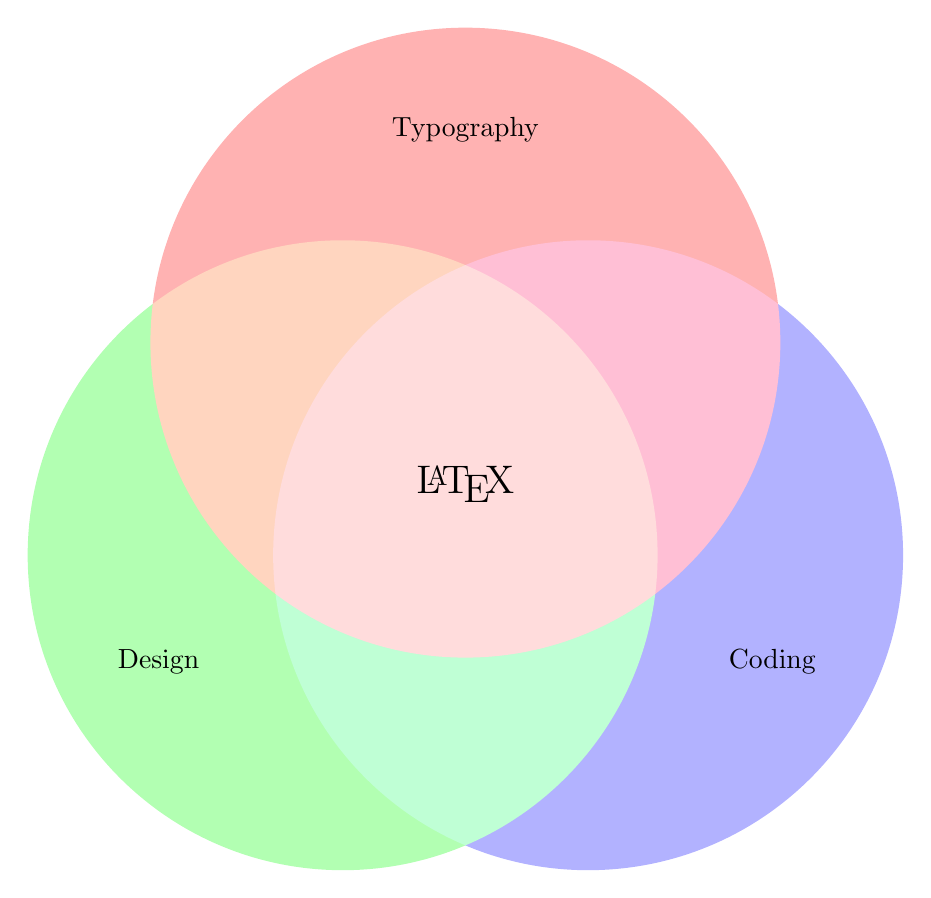
\begin{tikzpicture}
	\begin{scope}[blend group = soft light]
	\fill[red!30!white]   ( 90:1.8) circle (4);
	\fill[green!30!white] (210:1.8) circle (4);
	\fill[blue!30!white]  (330:1.8) circle (4);
	\end{scope}
	\node at ( 90:4.5)    {Typography};
	\node at ( 210:4.5)   {Design};
	\node at ( 330:4.5)   {Coding};
	\node [font=\Large] {\LaTeX};
	\end{tikzpicture}
	\caption{Test}
\end{figure}
\end{frame}

\begin{frame}{Block Test}
\begin{block}{Test}
This is a test block.
\end{block}
\vfill
\begin{definition}
This is a test definition.
\end{definition}
\vfill
\begin{theorem}
This is a test theorem.
\end{theorem}
\end{frame}

\end{document}


\section{Memory-Related Performance Problems}\label{sec:background}
Perhaps: \cite{tate2014programming,unat2017trends}

\subsection{Processor-Memory Speed Gap}\label{sec:pmgap}
\textit{Present the processor-memory speed gap. Explanation, why it is a problem will }

\subsection{Computation and Memory Requirements}\label{sec:comp_mem_req}
\textit{Present that requirements are increasing rapidly based on examples like ChatGPT, etc. -> There is always a need for more memory and more computation power}

\subsection{Data Transfer Costs and Bottlenecks}\label{sec:data_transfer}
\textit{Explain what common data transfer costs are (move from memory to caches and in between caches) and briefly explain bottlenecks (e.g. Cache misses, memory bandwidth, etc.)}

\subsection{Data Locality}\label{sec:data_locality}
\textit{Explain/Define the term data locality}

\section{Data Gathering and Visualization Approaches}\label{sec:methods}
In the pursuit of optimizing a program's data locality, implementing visual aids to represent data movements and data layouts can be particularly helpful. This approach enables quick and effective identification of data-related issues, their comprehension, and ultimately, their resolution. This method empowers not only program optimization experts but also domain researchers to effortlessly optimize their programs.

To enable such effective visualization, however, it's essential to first collect information regarding data locality. Several studies have explored this area, leading to the identification of three primary strategies: Dynamic Analysis, Static Analysis, and Simulation. These strategies, which we'll delve into in Sections \ref{sec:dynamic_analysis}, \ref{sec:static_analysis}, and \ref{sec:simulation}, each bring their unique benefits and drawbacks. Furthermore, it's important to note that some techniques used for gathering data locality information may not be confined to just one of these three fundamental categories, and could instead exhibit characteristics of multiple approaches.

Once this data locality information is gathered, it needs to be presented in a user-friendly manner. There exists a wide variety of visualization techniques that can fulfill this requirement, some of which we will detail in Section \ref{sec:visualization}.

\subsection{Dynamic Analysis}\label{sec:dynamic_analysis}
Dynamic analysis of a program's data locality involves executing the program while concurrently gathering memory-related data and statistics. A straightforward approach to dynamic analysis is to run the program, extract hardware counters such as cache misses, and analyze them. This approach, however, does not provide a holistic view of the program's behavior because it lacks contextual information.

To gain a deeper understanding of program performance beyond general statistics, dynamic analysis uses more nuanced techniques like profiling, statistical sampling, and tracing \cite{shende1999profiling,itzkowitz2003memory,gimenez2017memaxes,mckinley1999quantifying,adhianto2010hpctoolkit}.

Profiling involves periodically interrupting the program's execution to capture both hardware-derived attributes and context-related information \cite{itzkowitz2003memory,gimenez2017memaxes,adhianto2010hpctoolkit}. Profiling techniques analyze the program's call stack and program counter to provide specific details such as the current line of code being executed, the symbol, and, for arrays, the accessed index. This information facilitates the derivation of deeper metrics, such as the number of cache misses per array \cite{adhianto2010hpctoolkit}. Profiling typically focuses on memory-related events, but the constant interruption can increase runtime overhead. Hence, a trade-off between the granularity and the quality of the measurements is necessary.

Statistical sampling is an alternative approach related to profiling. It captures the program's state at fixed time intervals rather than event-triggered interruptions. The advantage of statistical sampling is that it avoids frequent interruption of the program's execution, reducing the runtime overhead. However, high-quality measurements require sufficiently high sampling rates to capture all relevant details \cite{adhianto2010hpctoolkit}.

Tracing, another technique, allows for a temporal understanding of a program's behavior by logging event-specific data over time. Tracing functions by documenting specific events or functions during program execution, providing a chronological account of these events and their corresponding data \cite{shende1999profiling,adhianto2010hpctoolkit,mckinley1999quantifying}.

In conclusion, dynamic analysis offers several distinct advantages in the study of a program's behavior concerning data locality. As the program is being executed, it offers more precise practical insights into hardware oriented data locality optimization. Further, dynamic analysis can be employed in conjunction with actual data, making it more representative of real-world scenarios.

However, it's important to note the inherent disadvantages of dynamic analysis. The act of running an entire program can be time-consuming and costly, particularly for larger and more complex software. Additionally, isolating and scrutinizing specific parts of a program under the dynamic analysis approach can be complicated, especially when compared to static analysis methods (Section \ref{sec:static_analysis}).

\subsection{Static Analysis}\label{sec:static_analysis}
Unlike dynamic analysis, static analysis takes a different tack in examining a program's data locality. Instead of operating the program in real-time to gather data, static analysis scrutinizes the program's source code itself. By transforming the source code into an intermediate representation (IR) that centers on data, and subsequently analyzing this IR, static analysis is able to uncover memory-related issues \cite{schaad2022boosting,schaad2021boosting,calotoiu2022lifting,ben2023bridging}.

There are myriad IRs in use, like MLIR, which are predominantly control-flow oriented, facilitating optimizations pivoting around control elements like loop restructuring \cite{moses2021polygeist}. However, in the context of data locality, data-centric IRs such as SDFG (\cite{ben2019statefulSDFG}), PROGRAPH (\cite{matwin1985prograph}), and LabVIEW (\cite{kodosky2020labview}) provide a more direct approach. By prioritizing memory, its movements, and its computation-induced alterations, these IRs allow for both automated (\cite{ben2019statefulSDFG}) and, when paired with visual aids, manual enhancements of data locality \cite{ben2023bridging,ben2019statefulSDFG,schaad2021boosting}.

\begin{figure}
  \centering
  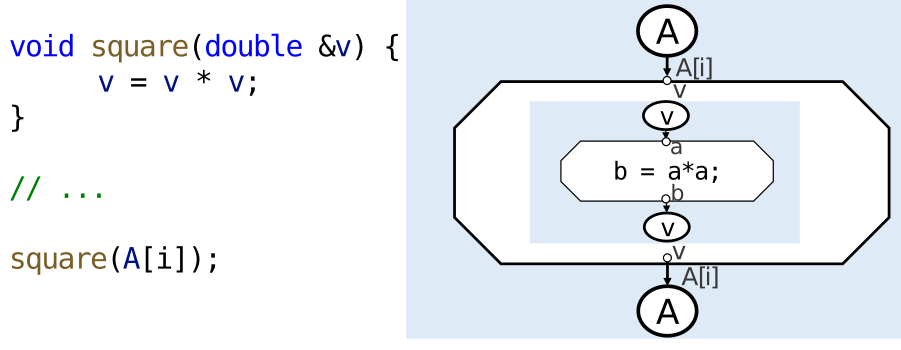
\includegraphics[width=\linewidth]{pictures/SDFG.png}
  \caption{C language source code and its corresponding SDFG representation \cite{calotoiu2022lifting}.}
  \label{fig:sdfg}
\end{figure}

Taking the example of SDFGs, the entire data flow of a program can be represented as a directed graph. Nodes within this graph symbolize $N$-dimensional arrays of data, computations (tasklets), or map scopes that denote general parallelism (such as loops). The edges, or memlets, in an SDFG represent explicit data movements \cite{ben2019statefulSDFG}. An example of the SDFG IR is provided in Figure \ref{fig:sdfg}.

As the SDFG IR of a program is constructed, it is possible to compute memory-related properties crucial for data locality. For instance, each memlet carries information regarding the volume of data transported between nodes \cite{ben2019statefulSDFG}, and tasklets and nested SDFGs can be annotated with metadata related to the number of executions and arithmetic operations undertaken \cite{schaad2021boosting}. Consequently, SDFGs offer a comprehensive view of the program and facilitate the identification of data movement bottlenecks on a large scale.

Despite static analysis's robust capability for macroscopic program analysis - a trait not shared with dynamic analysis - it does not provide the same level of detail. Given that performance bottlenecks are often induced by memory accesses that are tied to physical access patterns and hence are hardware-specific, static analysis alone may not accurately predict, say, the number of cache misses for a particular function. However, the advantage of static analysis lies in the fact that it does not necessitate program execution, thereby enabling quicker and cost-effective optimization of logical data movements compared to dynamic analysis.

\subsection{Cache Simulation}\label{sec:simulation}
Positioned between dynamic and static analysis lies the realm of simulation-based approaches, of which cache simulation is particularly noteworthy. Cache simulation is a method used to simulate a program's data accesses on a virtual memory hierarchy model. This process allows for an in-depth examination of both spatial and temporal data locality, as elaborated on in Section \ref{sec:data_locality}.

The process of setting up a cache simulator can be divided into two ways:

In the first approach, the program is pseudo-executed without implementing any real computations. This process starts by constructing a virtual memory hierarchy that includes caches. As the program proceeds through its lifecycle:
\begin{itemize}
	\item Corresponding space is allocated in the simulated memory for each instance of allocation, and reciprocally, space is deallocated as per the program's instructions.
	\item The simulator emulates each memory access operation, both read and write, according to how a CPU would handle the task. This entails an initial probe in the L1 cache, followed by a potential cache miss procedure if the required data is absent, as discussed in Section \ref{sec:data_transfer}.
\end{itemize}
This methodology facilitates a comprehensive and accurate representation of the system's memory hierarchy and its interaction with the computing process \cite{schaad2022boosting,hammer2017kerncraft}.

The second approach uses dynamic analysis (Section \ref{sec:dynamic_analysis}) to generate memory traces. These traces are then rerun through the simulator, enabling an enriched understanding of memory access and management behavior within the program \cite{choudhury2011abstract}.

The deployment of cache simulators extends beyond mere prediction of cache misses. When operated in a step-by-step manner, these tools permit the exploration of data access patterns of a procedure at a granular level. Such detailed inspection can uncover potential enhancements in spatial locality, either through modifications in data layout or access strategies, ultimately contributing to improved performance \cite{schaad2022boosting,hammer2017kerncraft,choudhury2011abstract}.

Moreover, cache simulation enables close-up performance analysis of a program, such as focusing on a single function within the source code or limiting memory traces to a specific functional context.

Despite its advantages, cache simulation demands an in-depth understanding of the target architecture, including aspects like cache hierarchy, cache replacement policy, and cache coherence protocol. Any inaccuracies in these parameters can lead to misleading results, potentially causing optimization attempts to inadvertently degrade the program's data locality.

\subsection{Visualization Techniques}\label{sec:visualization}

\subsubsection{Coarse View}

\subsubsection{Medium View}

\subsubsection{Fine-Grained View}

\textit{Very brief overview of different visualizations (Colored Graphs, Heatmaps, etc.)}

\textit{From HPC Toolkit: Typical metrics such as elapsed time
are useful for identifying program hot spots. However, tuning a program usually requires a measure
of not where resources are consumed, but where they are consumed inefficiently. For this purpose,
derived measures such as the difference between peak and actual performance are far more useful than
raw data such as operation counts. HPCTOOLKIT’s hpcviewer user interface supports computation
of user-defined derived metrics and enables users to rank and sort program scopes using such metrics.}

\section{Exemplary Memory Access Visualization Tools}\label{sec:works}

This section examines several prominent works dedicated to visualizing memory movements and accesses. Each tool will be discussed in terms of its data gathering methods, visualization techniques, and demonstrated results. We will then contrast these tools, highlighting their strengths and weaknesses.

\begin{figure*}
	\begin{subfigure}[c]{.48\linewidth}
		\centering
		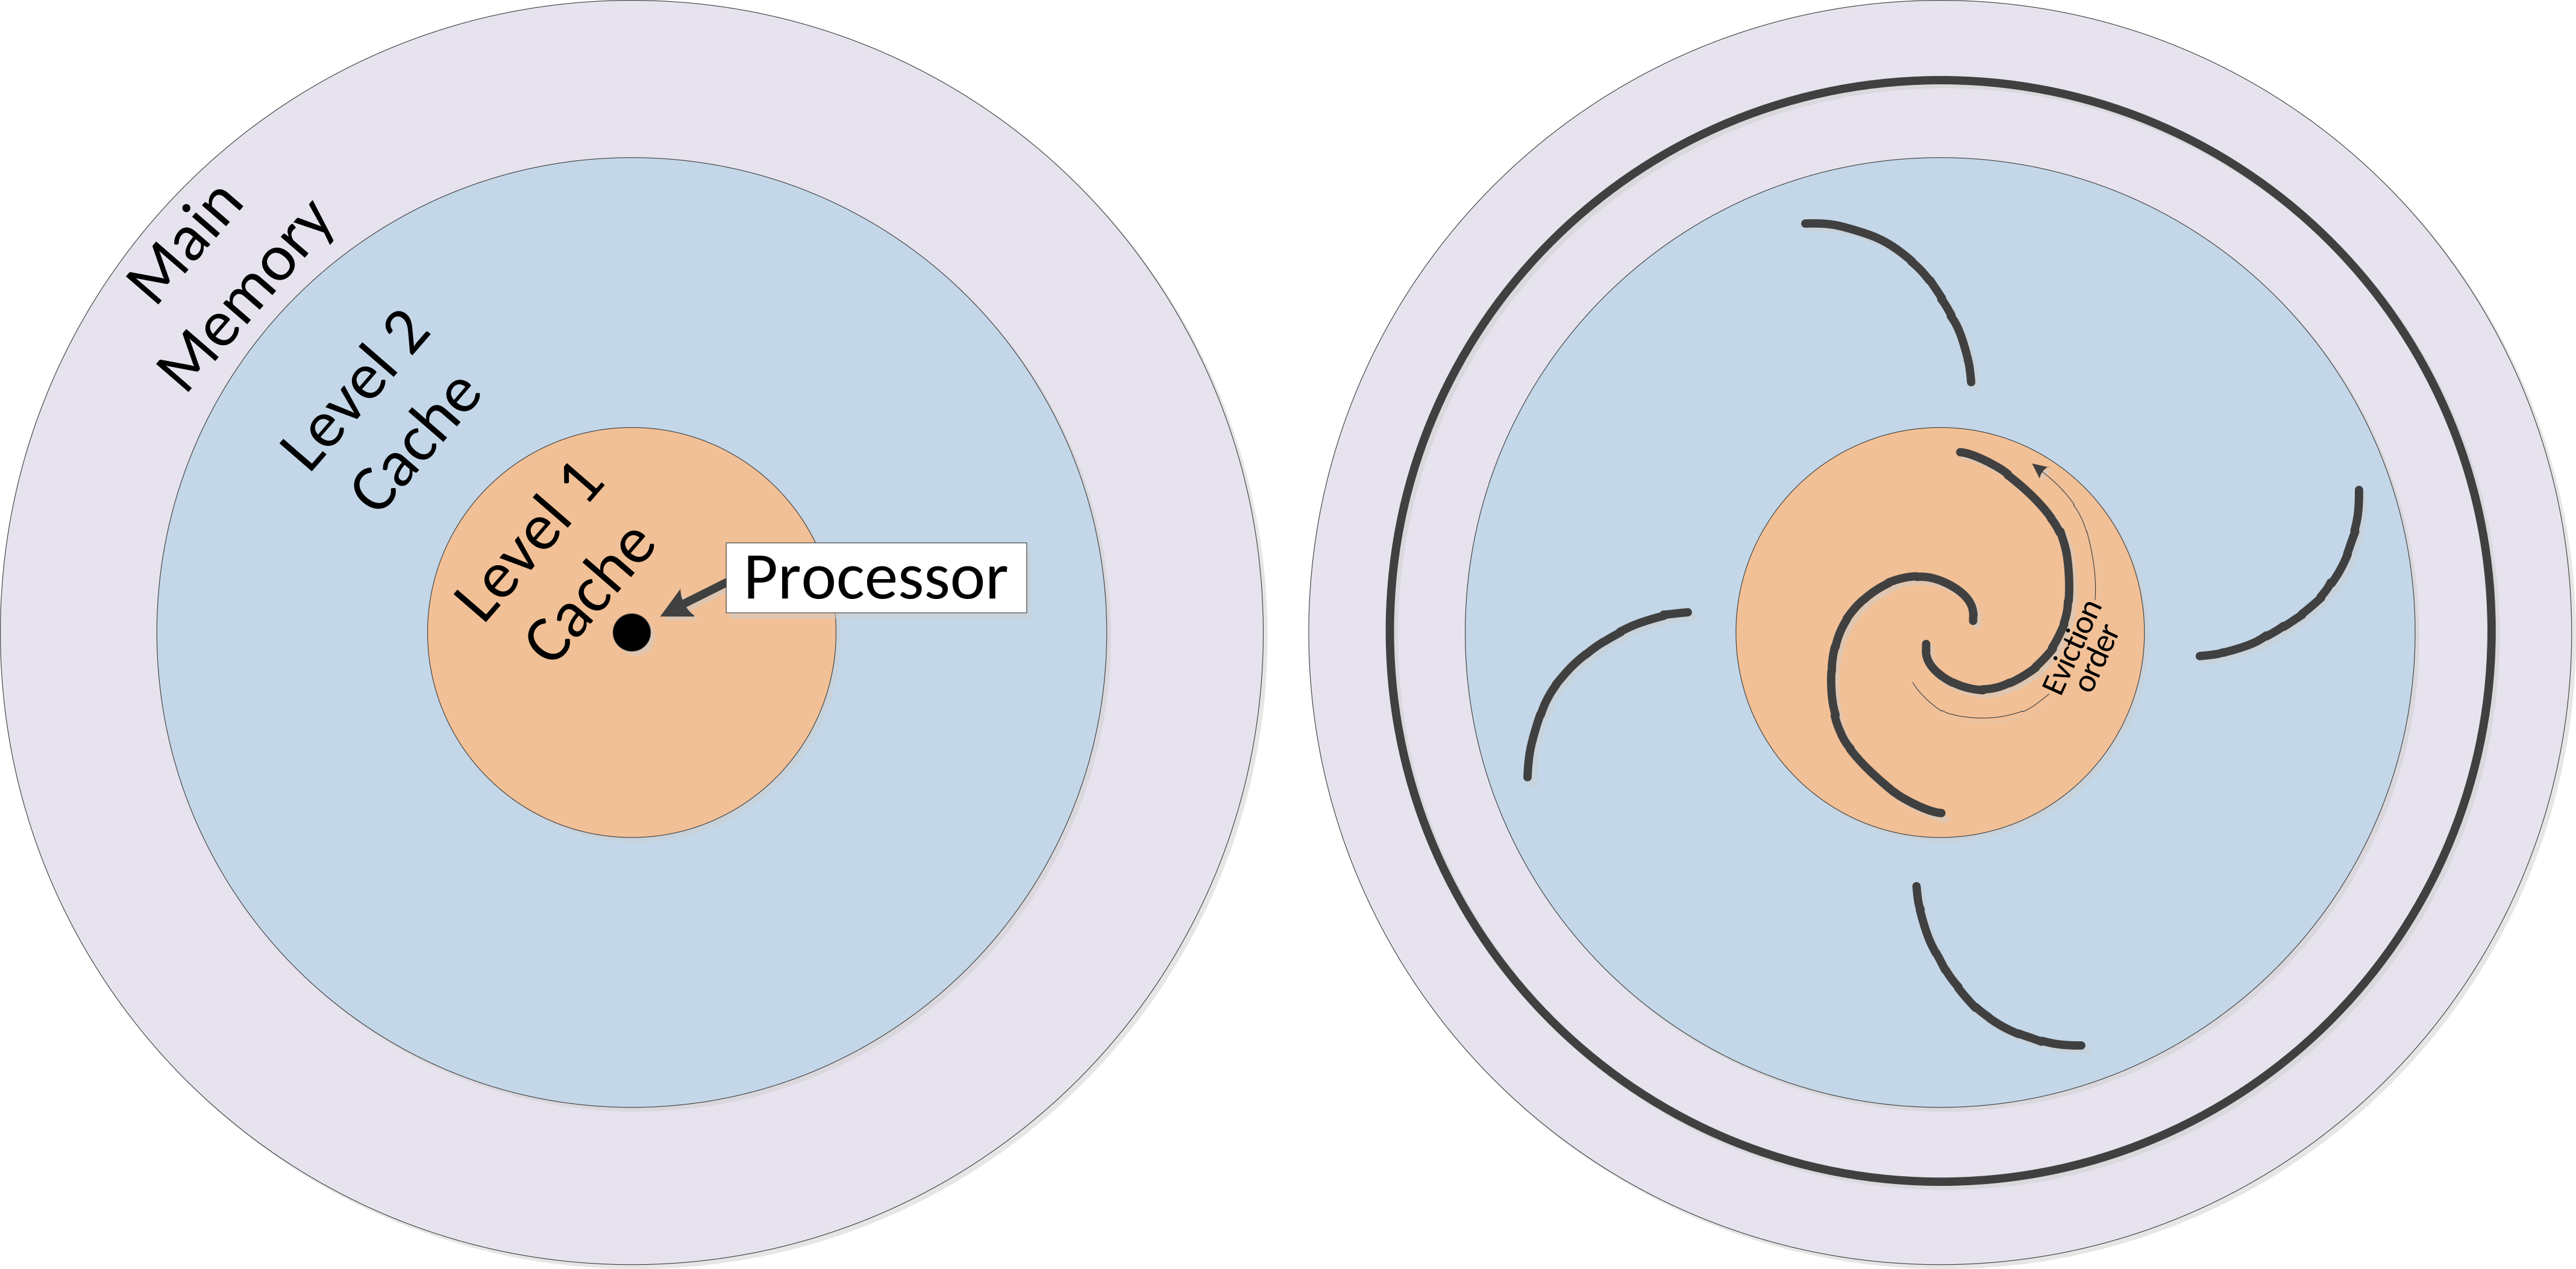
\includegraphics[width=\linewidth]{pictures/abstract_explanation.png}
	\end{subfigure}
	\begin{subfigure}[c]{.24\linewidth}
		\centering
		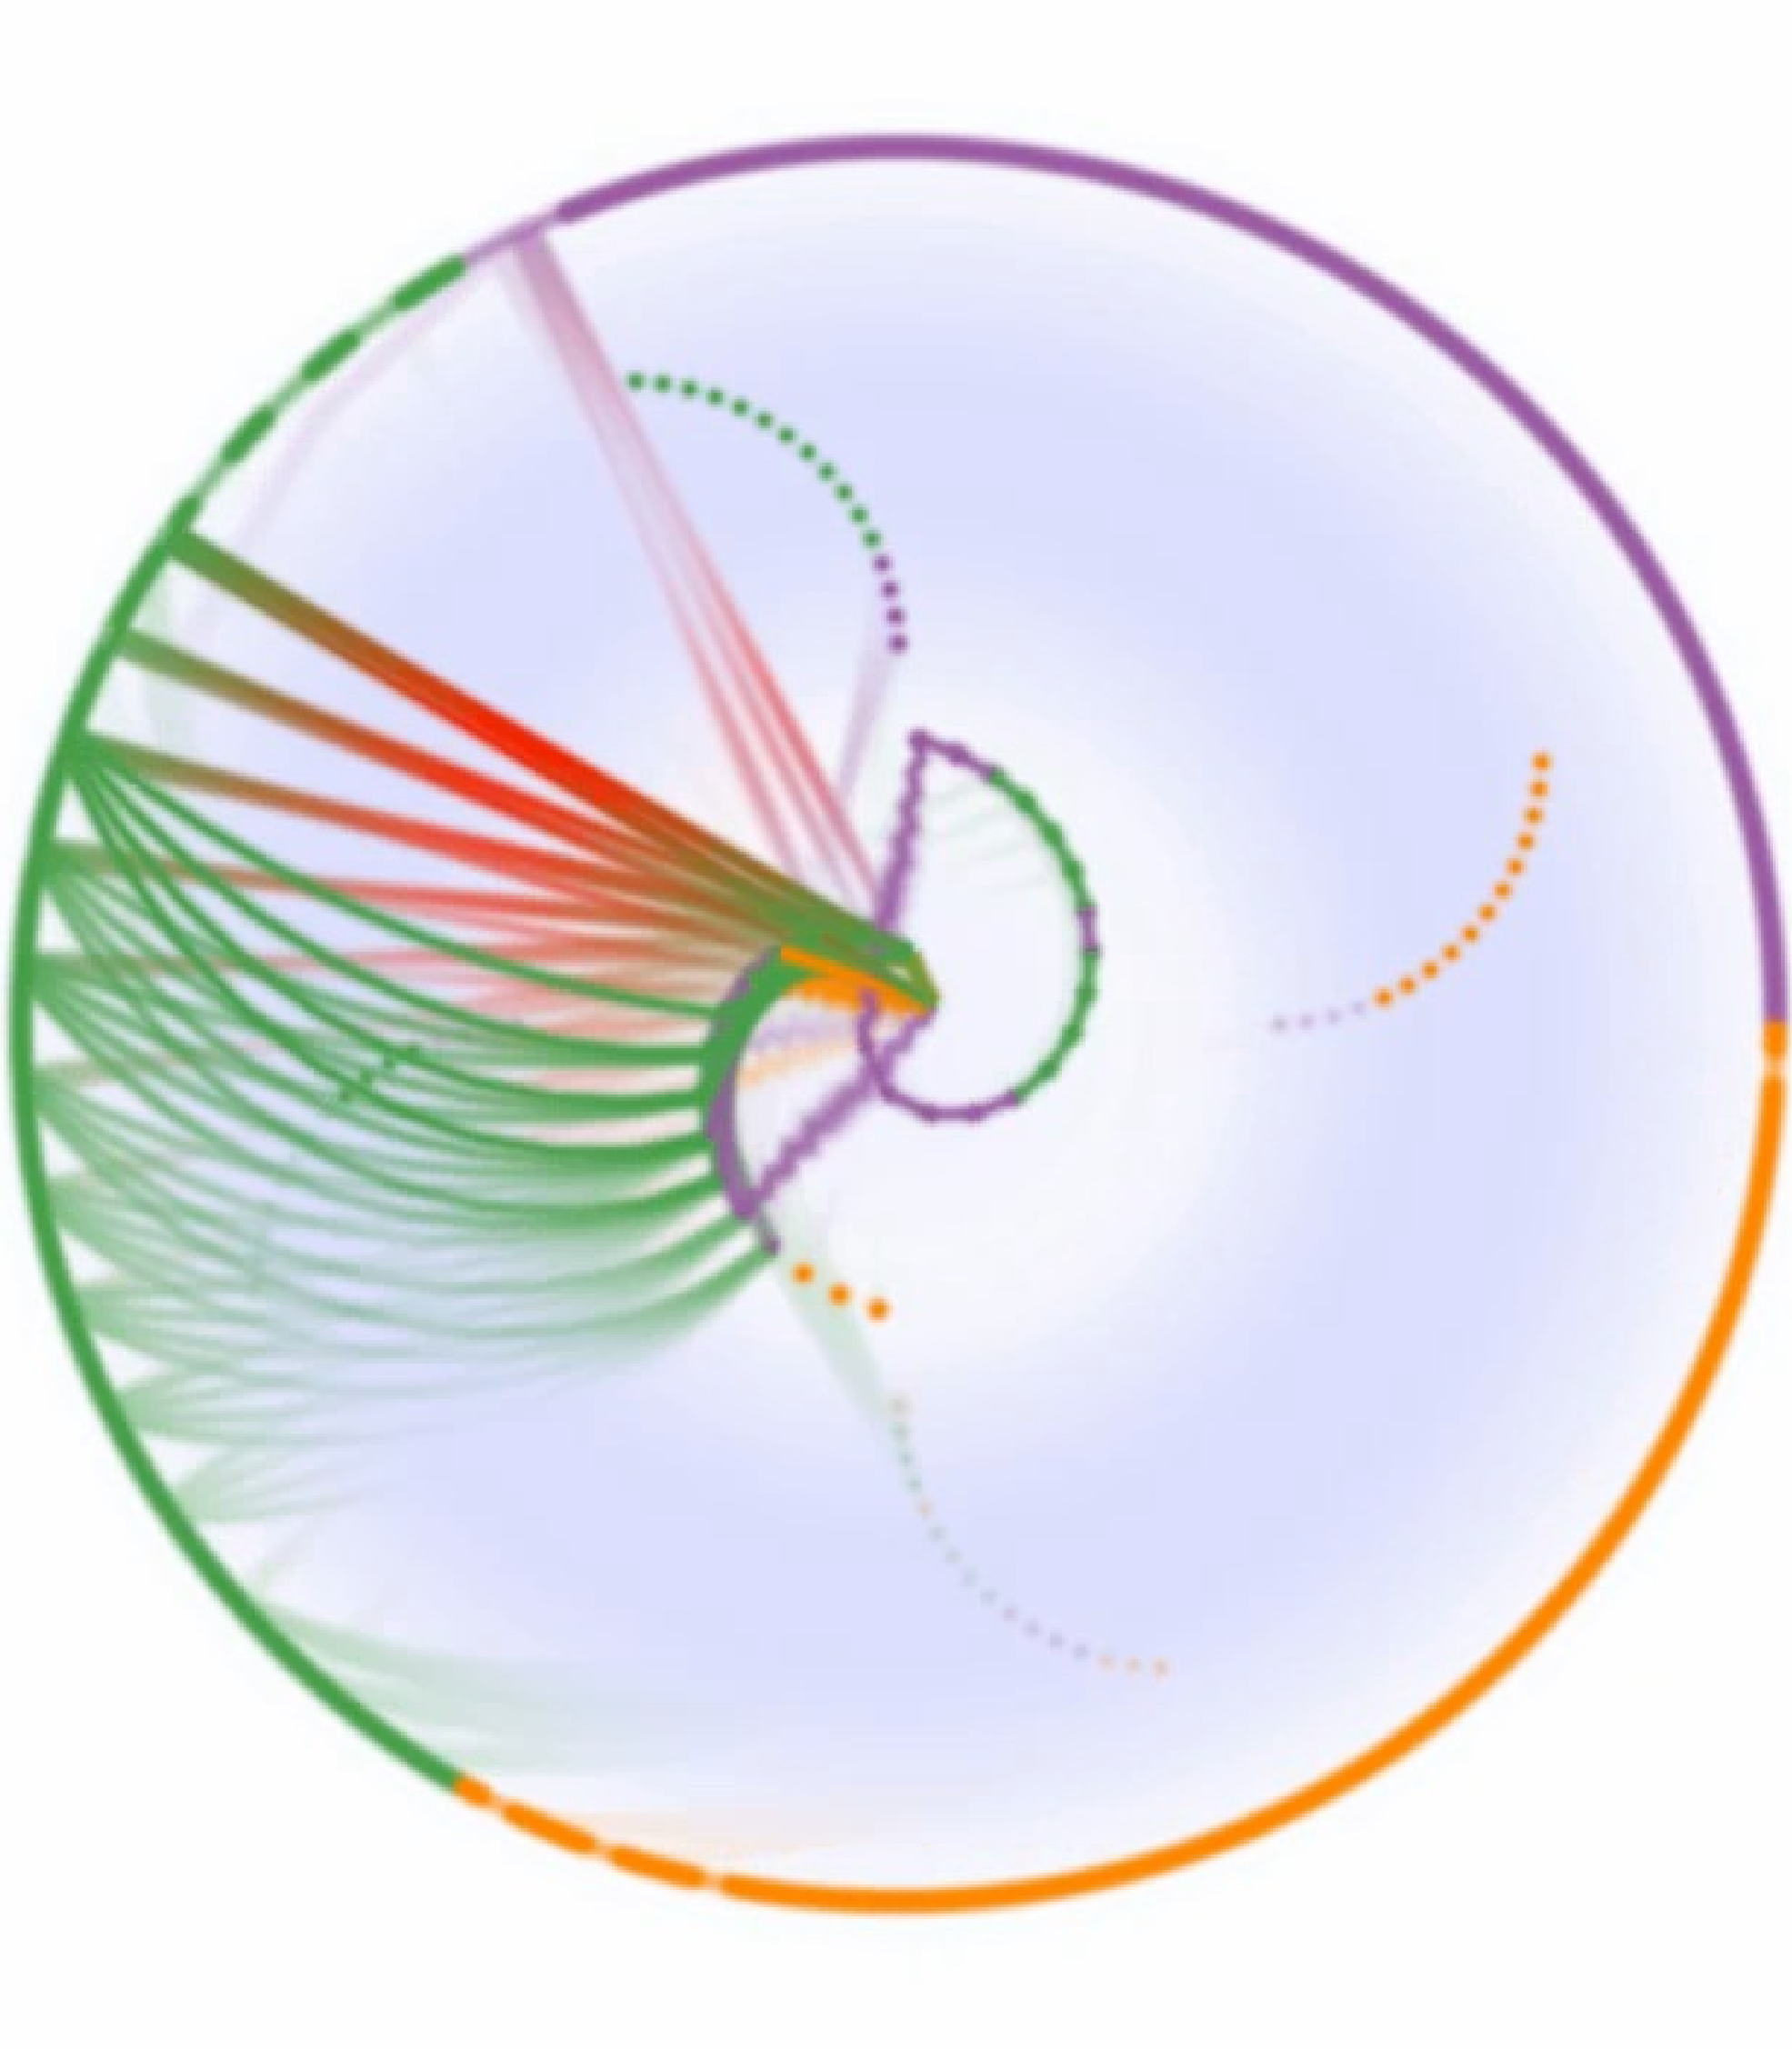
\includegraphics[width=\linewidth]{pictures/abstract_standard.png}
	\end{subfigure}
	\begin{subfigure}[c]{.24\linewidth}
		\centering
		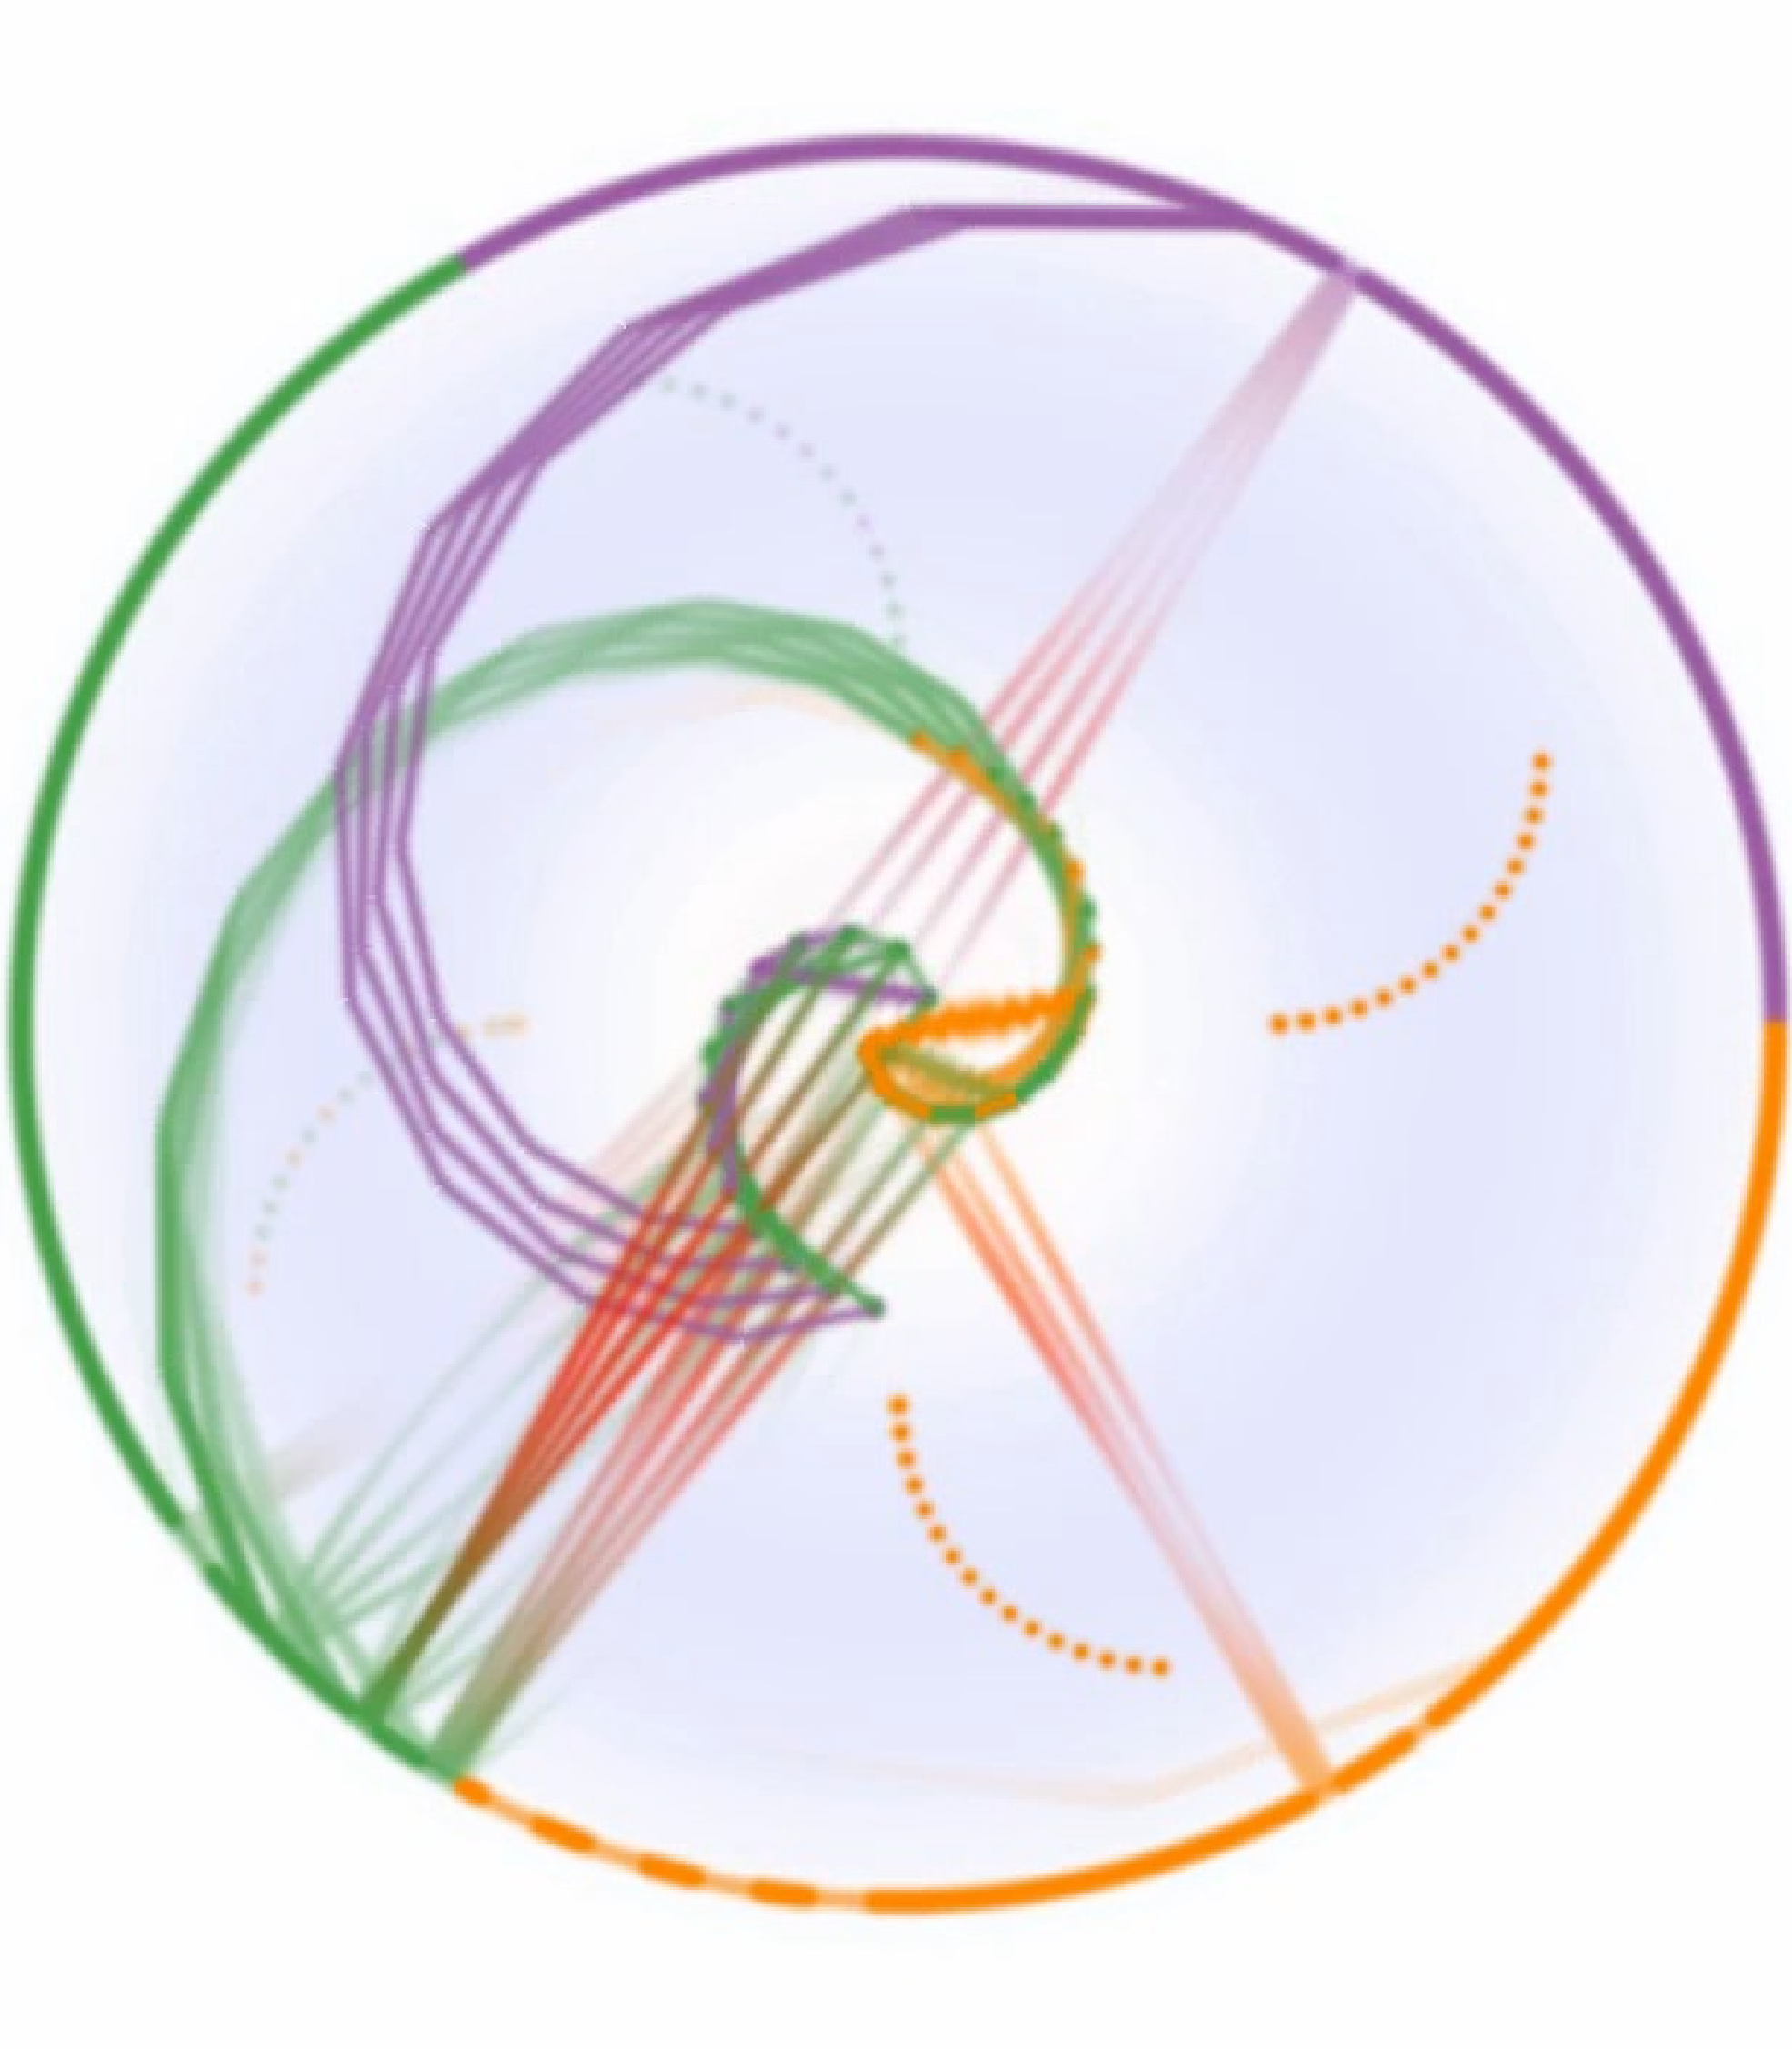
\includegraphics[width=\linewidth]{pictures/abstract_optimized.png}
	\end{subfigure}
	\caption{Left: Radial design used in \cite{choudhury2011abstract}. Glyphs arrange themselves into groupings indicating storage on the same cache, with data closer to the boundaries between the levels more likely to be evicted. Right: A comparison of a standard $16 \times 16$ matrix multiplication and an optimized version using $4 \times 4$ blocking. The standard version shows poor data reuse for two of the three matrices \cite{choudhury2011abstract}.}
	\label{fig:abstract_cache}
\end{figure*}

\subsection{MemAxes: Visualization and Analytics for Characterizing Complex Memory Performance Behaviors}\label{sec:memaxes}
The tool \texttt{MemAxes}, developed by Giménez et al. \cite{gimenez2017memaxes}, utilizes dynamic analysis (Section \ref{sec:dynamic_analysis}) to generate an event log of memory accesses. Each logged event incorporates contextual information, facilitating a link back to the source code and recording the memory hierarchy depth at which the memory access occurred. This feature allows for the identification of problematic code lines, similar to \texttt{HPCToolkit} \cite{adhianto2010hpctoolkit}, as illustrated in Figure \ref{fig:coarse}. Recording the resolution depth of memory access enables the determination of resource utilization across each memory module and the quantification of physical data movements between them. This information is then visualized using a radial design of the hardware topology, as seen in Figure \ref{fig:memaxes_cache}. \texttt{MemAxes} also supports the display of additional attributes such as access times, latencies, and memory addresses through histograms.

In practical applications, \texttt{MemAxes} has been employed successfully to detect and mitigate performance bottlenecks, even without prior knowledge of the application's source code \cite{gimenez2017memaxes}. Performance engineers can, for instance, identify large load imbalances or significant spikes in access times, and use these insights to hypothesize the cause of a performance bottleneck. This hypothesis can then be explored further through the backlink to the source code. This approach demonstrates that low-level visual aids are not necessary for optimizing data locality in an unfamiliar program.

\subsection{Abstract Visualization of Runtime Memory Behavior}\label{sec:abstract}

Choudhury et al. \cite{choudhury2011abstract} offer a unique perspective on runtime memory behavior through their visualization tool, conceptually different from \texttt{MemAxes}. Their approach involves dynamic analysis to chronicle an event log of memory accesses during runtime (Section \ref{sec:dynamic_analysis}), which then feeds a cache simulator (Section \ref{sec:simulation}). The output is a series of radial visualizations, exemplified in Figure \ref{fig:abstract_cache}, which are generated throughout the program's execution, forming an animation of evolving data movements within the memory hierarchy.

The visualization in Figure \ref{fig:abstract_cache} uses a concentric layout to demonstrate memory usage patterns. Glyphs, symbolizing memory locations, navigate across layers representing main memory and different cache levels. Movements towards the center imply recent references, while those towards the periphery indicate aging or eviction. Performance issues, such as inefficient memory usage or frequent evictions, are suggested by rapid, large-distance glyph movements. Conversely, slow in-layer movement indicates high cache hits, signaling efficient memory utilization \cite{choudhury2011abstract}.

Choudhury et al. argue that this dynamic approach is more intuitive than static visualizations, such as those provided by \texttt{MemAxes}, as it presents an overview of large-scale memory access and caching behavior. However, its granularity is insufficient for targeted bottleneck resolution, given that the visualizations lack linkage to specific contextual information such as precise addresses or lines of code.

\subsection{Boosting Performance Optimization with Interactive Data Movement Visualization}\label{sec:boosting}
The tool developed by Schaad et al. \cite{schaad2021boosting,schaad2022boosting} enables two-tier program analysis:

At the global level, static analysis (Section \ref{sec:static_analysis}) is used to compile the program source code into an SDFG graph, providing an overview as shown in Figure \ref{fig:coarse}. This graph, with its color-customizable nodes and edges, aids in identifying problematic program sections, especially when utilizing the automatic node and edge collapsing feature for easy zooming.

For in-depth analysis of data locality and reuse behavior, the tool uses cache simulation (Section \ref{sec:simulation}) to offer detailed views of specific program segments, as depicted in Figure \ref{fig:boosting_cache}.

The authors successfully employed this tool to significantly optimize two applications. After pinpointing problem areas in the global view, the engineers utilized the local view for a thorough investigation and subsequent optimization of these areas.

\subsection{Comparison}\label{sec:comparison}
Among the three tools, the animation provided by Choudhury et al. \cite{choudhury2011abstract} offers the most intuitive understanding of large-scale memory access and caching behavior. However, comprehensive program optimization requires contextual information about inefficient memory access locations, which is supplied by \texttt{MemAxes} \cite{gimenez2017memaxes} and the tool by Schaad et al. \cite{schaad2021boosting}. Of all three, Schaad et al.'s tool provides the most detailed low-level visualizations. The tool's ability to depict the influence of data layout on the cache hit ratio proves invaluable for optimizing data locality. However, the tool's reliance on cache simulation necessitates consideration of parameterization, as discussed in Section \ref{sec:simulation}.

\section{Conclusions}
This paper provided a comprehensive exploration of the different methodologies employed to understand and visualize data movements and accesses in computer programs, an imperative for optimizing performance. The data acquisition processes are based on three principal methodologies, which can often be combined to achieve a more comprehensive analysis. Dynamic Analysis, involving the execution of a program to gather data, provides accurate results, albeit time-consuming. Static Analysis, on the other hand, is a swift method that just analyzes the source code, bypassing the need for program execution, but can sometimes produce insufficient insights. Lastly, Cache Simulation offers an in-depth understanding of a program's interaction with the memory hierarchy, allowing for a meticulous examination of its performance.

Once the data locality information is collected, it becomes essential to present it in an intuitive yet informative way. Here, visualizations play a critical role. These visualizations, varying in their granularity, offer insights into different levels of the program, from high-level overviews to fine-grained dissections of memory usage. The use of multiple visualizations in tandem empowers performance engineers to gain a comprehensive understanding of data movements and accesses, leading to effective bottleneck resolution.

In this regard, we delved into three prominent works that provide unique tools for visualizing data movements and accesses. Each work was presented and compared, highlighting their distinctive contributions to the wider landscape of methods employed in this domain.

The broad-ranging implications of these methods were underscored, highlighting their relevance to not just high-performance computing (HPC) but to any application that would benefit from performance optimization. This paper thus provides a solid foundation for understanding and visualizing data movements and accesses, a crucial aspect of programming and performance engineering.

As we look to the future, the field holds exciting prospects. The continuous refinement of data gathering methods and visualizations is one aspect, but the ultimate goal extends to automatic program optimization. Initiatives have already been launched to develop algorithms for automatic optimization \cite{calotoiu2022lifting}, significantly easing the programmer's workload. Such advancements could be especially beneficial for domain researchers, allowing them to focus more on their domain-specific work.

The emergence of machine learning, particularly deep learning, also presents new avenues for program optimization. Preliminary work in this area indicates that future compilers might utilize machine learning for automatic, compile-time program optimization \cite{cummins2021programl}.

In conclusion, the tools and methods presented in this paper provide a solid foundation for understanding and visualizing data movements and accesses, a crucial aspect of optimizing program performance. With ongoing advancements in automatic program optimization and the advent of machine learning techniques, the future looks bright for further improvements in this vital aspect of programming and performance engineering.


% Print references
% Add entries to "literature.bib"
\printbibliography

\end{document}